%\documentclass{amsart}

\documentclass{article}
\usepackage[a4paper,hmargin=15mm,vmargin=20mm]{geometry}
\usepackage[nosetup, colorlinks]{tony}
\usepackage{graphicx}

\usepackage{mathpazo}
\usepackage{amsmath}
\usepackage{multicol}
\usepackage{diagbox}


\title{6.867: Problem Set 1}
\author{Benjamin Bitdiddle, and Hacker, A.}
\date{September 29, 2016}

\begin{document}

%\begin{abstract}
%% #PLACEHOLDER
%MY ABSTRACT HERE summary summary
%\end{abstract}

\maketitle

\begin{multicols}{2}
% % % % % % % % % %
%    PROBLEM 1
% % % % % % % % % %

\section{Gradient Descent}

\subsection{Batch Gradient Descent}

We implemented a general-purpose batch gradient descent as described in Bishop 5.2.4, with user-specified objective function and gradient thereof, initial guess, step size, and termination criterion. % TODO elaborate on this?
We tested our implementation against two functions: a sign-reversed multivariate Gaussian with mean~$\mu$ and covariance matrix~$\Sigma$
\begin{equation}
f(x; \mu, \Sigma) = -\frac{e^{-\frac12(x - \mu)^T \Sigma^{-1}(x - \mu)}}{\sqrt{(2\pi)^n \det\Sigma}}
\end{equation}
and a quadratic bowl
\begin{equation}
f(x; A, b) = \frac{1}{2}x^T Ax - x^T b,
\end{equation}
where $A$ is positive-definite. For this exercise, our Gaussian was tested with $\mu = (10, 10)^T$, $\Sigma = 1000 \cdot I_2$. For the quadratic bowl, we took \[A = \left(\begin{array}{cc}10 & 5 \\5 & 10\end{array}\right)\] and $b = (400, 400)^T$. Figure \ref{fig:1.1} illustrates the effect of the initial guess and step size for convergence given these values.

\begin{figure*}%  figure placement: here, top, bottom, or page
   \centering
   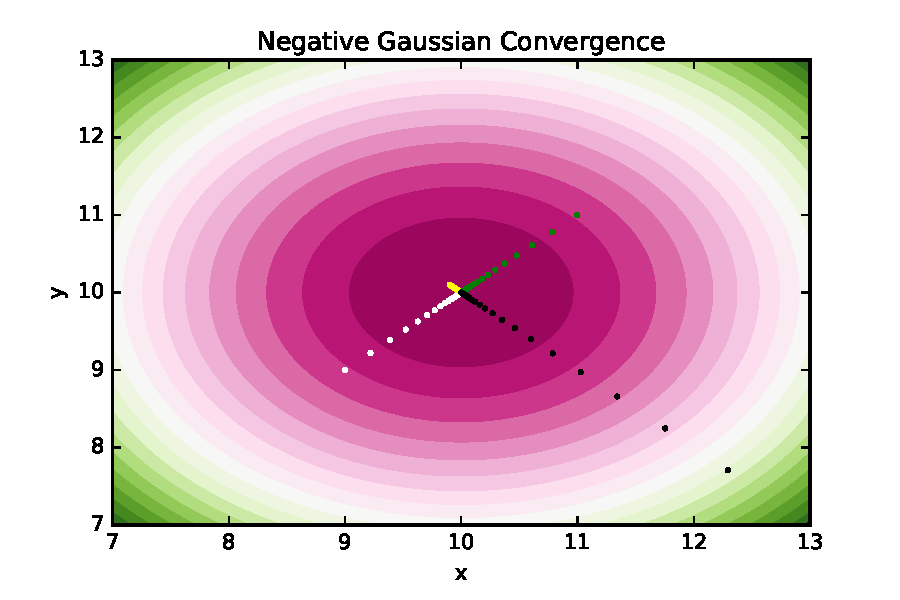
\includegraphics[width=3in]{img/1-1-gauss.pdf}  % $PLACEHOLDER
   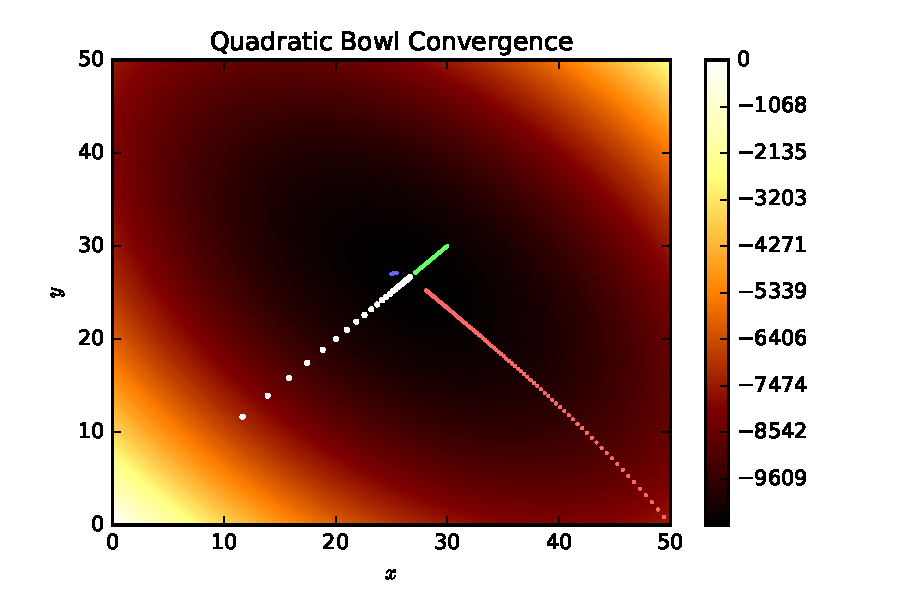
\includegraphics[width=3in]{img/1-1-quad.pdf}  % $PLACEHOLDER
   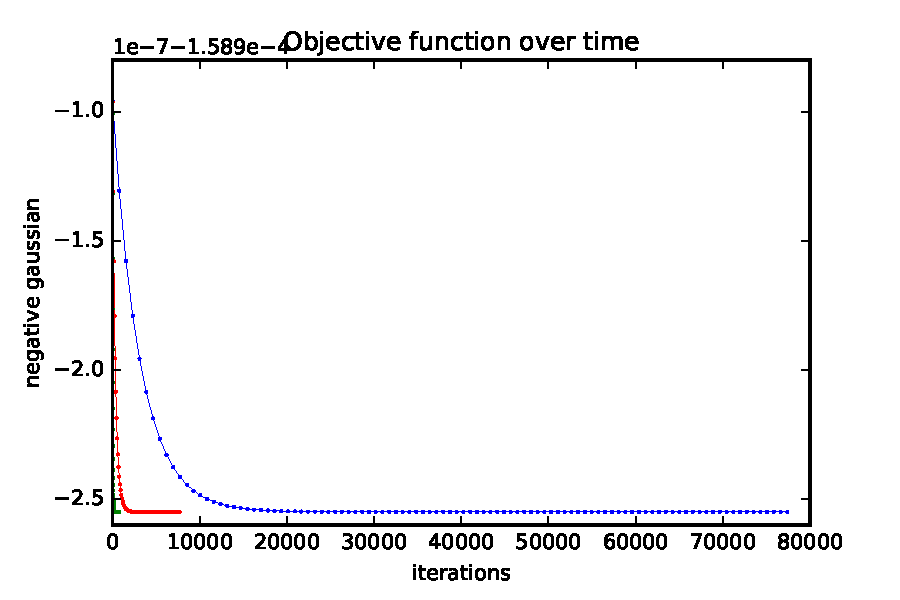
\includegraphics[width=3in]{img/1-1-etaGauss.pdf}  % $PLACEHOLDER
   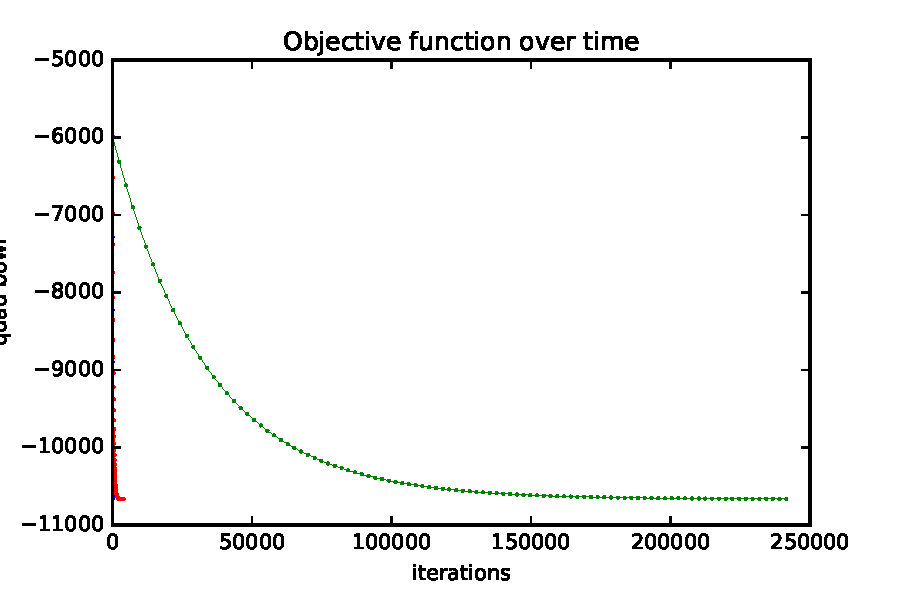
\includegraphics[width=3in]{img/1-1-etaQuad.pdf}  % $PLACEHOLDER
   \caption{Effects of initial guess and step size on convergence. Bad initial guesses took much longer to converge (8428 and 5743 iterations) than good initial guesses (6292 and 372 iterations, respectively). The bottom two figures show the change in objective function over time. Larger step sizes (red and green) also converged faster, if they converged at all.}
   \label{fig:1.1}
\end{figure*}

\begin{figure*}%  figure placement: here, top, bottom, or page
   \centering
   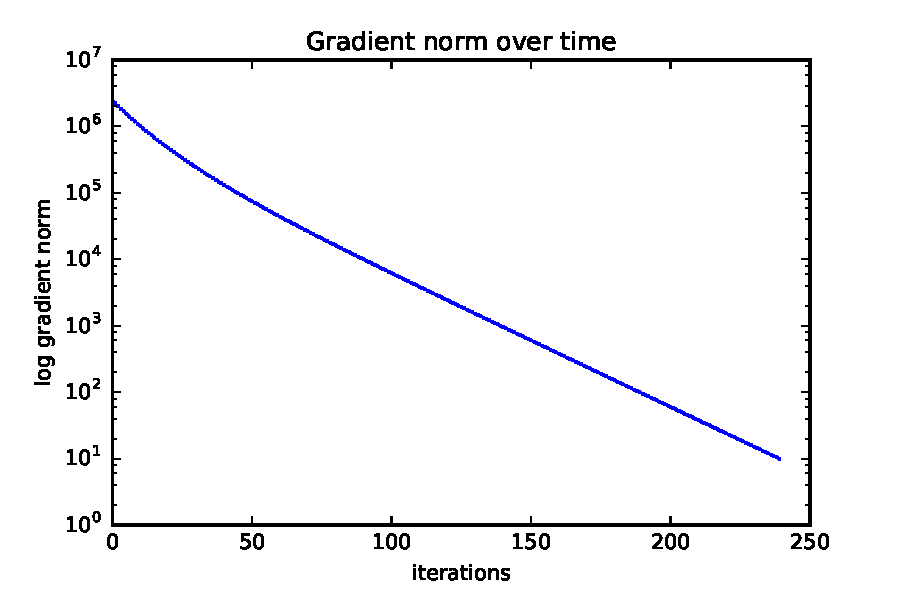
\includegraphics[width=3in]{img/1-1-batch.pdf}  % $PLACEHOLDER
   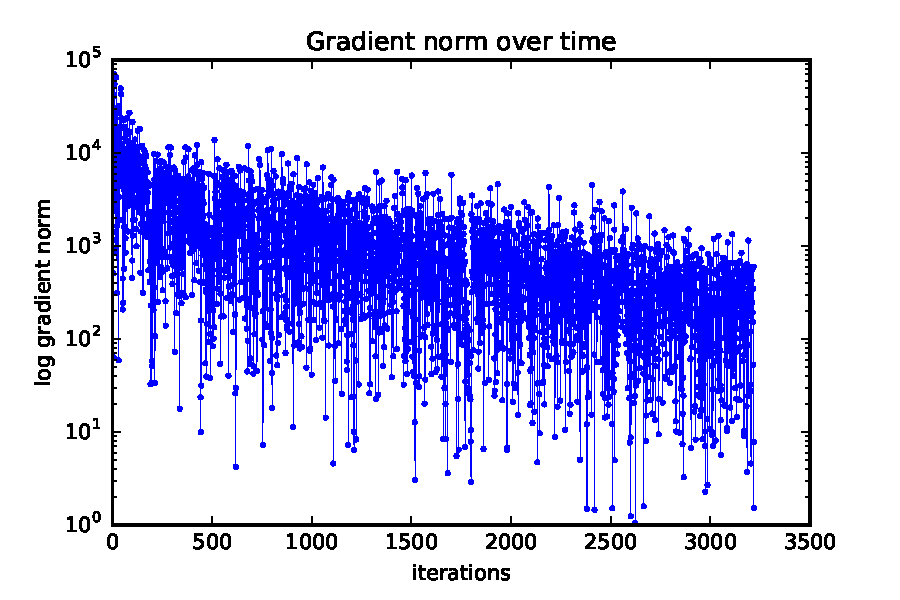
\includegraphics[width=3in]{img/1-1-stoch.pdf}  % $PLACEHOLDER
   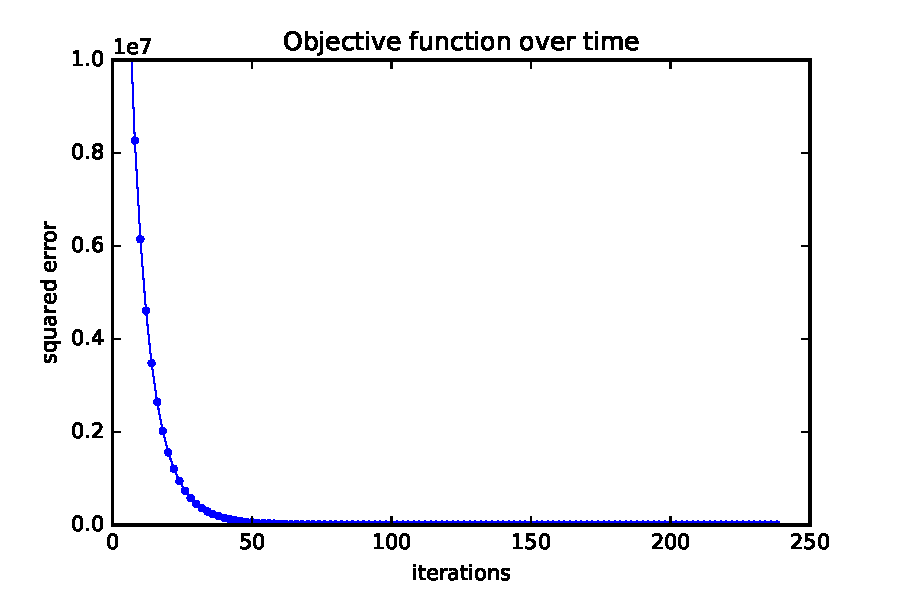
\includegraphics[width=3in]{img/1-1-batch-func.pdf}  % $PLACEHOLDER
   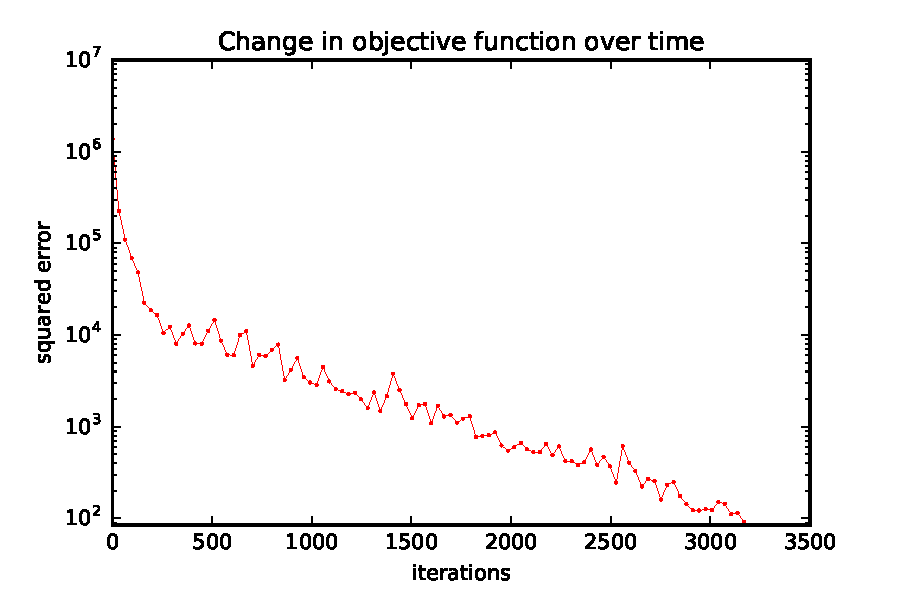
\includegraphics[width=3in]{img/1-1-stoch-func.pdf}  % $PLACEHOLDER
   \caption{Batch gradient descent (left) and stochastic gradient descent (right). We see that SGD descent requires more iterations to converge and fluctuates more, in both objective function and gradient, than BGD.}
   \label{fig:1.2}
\end{figure*}


% TODO Do something with this
% For the Gaussian, we had $\mu = (10, 10)^T$, $\Sigma = \left(\begin{array}{cc}1000 & 0 \\0 & 1000\end{array}\right)$. For the quadratic bowl, we had $A = \left(\begin{array}{cc}10 & 5 \\5 & 10\end{array}\right)$ and $b = (400, 400)^T$.

% #PLACEHOLDER
% TODO
% present results of experiments
% "Discuss (and illustrate) the effect of the choice of starting guess, the step size, and the convergence criterion on the resulting solution, as well as how the norm of the gradient evolves through the iteration.

\subsection{Numerical Gradient Approximation}
\label{subsec:grad-approx}

Recall that our gradient descent procedure requires the user to specify both the objective function \emph{and} its gradient. With our examples, these gradients had simple analytic forms, but such is not the case for general objective functions. Therefore, as a check on (or a substitute for) the user-specified gradient, we implemented a gradient approximation routine.

Our procedure approximates the gradient of a general function~$f:\RR^d\to\RR$ at some given point~$x^*$ by approximating its partial derivatives as the central difference
\begin{equation}
\label{eq:grad-approx}
\f{\pa f}{\pa x_i}(x^*) \approx \f{f(x^* + \f12\eps\hat x_i) - f(x^* - \f12 \eps\hat x_i)}{\eps},
\end{equation}
where $\eps > 0$ is some user-supplied small difference step and $\hat x_i$ is the unit vector in the $x_i$ direction. We compute this approximate partial derivative along each dimension of our domain and collect the terms into our numerical gradient approximation. 

% #PLACEHOLDER
% TODO
% "Verify the gradient values on the functions you used in the question above by comparing the closed-form and numerical gradients at various points. Discuss the effect of changing the difference step (or "delta") on the accuracy of the gradient evaluation."

Numerically we noted that the difference step produced the best guess when it was relatively close in order of magnitude to the points of interest. Too small a step resulted in rounding inaccuracies, while too large a step overstretched the assumption that the function could be approximated by a hyperplane at the point.

% this damn table disappears

%\begin{center}
%\begin{tabular}{|c|c|c|c|c|}\hline
%\label{tab:1.2}
%$\epsilon$ & 1000 & 100 & 10 & 1e-4 \\ \hline
%MSE & 2.0e-17 & 1.4e-18 & 3.8e-18 & 2.1e-12 \\
% \hline
%\end{tabular}
%\end{center}

\subsection{Stochastic Gradient Descent}

By design, batch gradient descent determines each update step by looking at the entire dataset and taking a gradient. This approach clearly becomes unfeasible with large datasets, and does not extend easily to online settings. For these reasons, we instead use stochastic gradient descent (SGD), in which we approximate the gradient as follows.

Suppose our objective function takes the form
\begin{equation}
J(\theta) = \sum_i J_i(\theta)
\end{equation}
where each $J_i$ is presumably a term corresponding to a single data point. Whereas the batch gradient descent update step takes a gradient over all $J$:
\begin{equation}
\theta_{t+1} = \theta_t - \eta \nabla J(\theta_t),
\end{equation}
the SGD update step has the form
\begin{equation} \theta_{t+1} = \theta_t - \eta_t \nabla J_i(\theta_t). \end{equation}

Note two key differences. We take $\nabla J_i$ as an approximation of $\nabla J$. More interestingly, our step size is now time-dependent. Because SGD is stochastic, it is unclear that SGD converges. But it can be shown that if we choose a learning rate schedule $\eta_t$ satisfying the Robbins-Monro conditions ($\sum_{t=1}^\infty \eta_t$ diverges and $\sum_{t=1}^\infty \eta_t^2$ converges), we get guaranteed convergence. Figure \ref{fig:1.2} illustrates that while SGD fluctuates during convergence, it eventually does converge, like BGD.

We implemented two stopping criteria: either gradient norm or change in objective function drop below a provided threshold. For these problems, we mostly utilized change in objective function.
% #PLACEHOLDER
% TODO describe specific problem
% TODO talk about learning rate schedule and stopping criterion we chose for specific problem
% TODO part 1c



% % % % % % % % % %
%    PROBLEM 2
% % % % % % % % % %

\section{Linear Regression}

Before we proceed, recall that a linear basis function model for a dataset $(x^{(n)},y^{(n)})$ given a fixed set of basis functions $\phi_i$ is a regression model that tries to find weights~$w_i$ for which we approximately have
\[ y^{(n)} = w_0 + \sum_i w_i \phi_i(x^{(n)}). \]
In other words, we transform the independent variable $x$ by basis functions~$\phi_i$, then perform linear regression with independent variables $\phi_i(x)$ and dependent variable~$y$.

We wrote a procedure for general linear basis function regression with user-specified data points and basis functions that found the maximum-likelihood weight vector analytically, via Bishop Equation 3.15, which we restate here:
\begin{equation}
\label{eq:max-likelihood-weights}
w_\tx{ml} = (\Phi^T\Phi)\inv\Phi^T Y
\end{equation}
where $Y$ is a vector of $y^{(n)}$ values from our dataset and $\Phi$ is the design matrix, given by
\begin{equation}
\Phi_{ij} = \phi_j(x^{(i)}).
\end{equation}

\subsection{Polynomial Basis Functions}

We tested our procedure by performing fits on a dataset of 11 points with polynomial basis functions up to some specified degree $M$. The dataset was generated by applying noise to the values produced by the function
\begin{equation}
\label{eq:dataset-secret-func}
y(x) = \cos(\pi x) + \cos(2\pi x).
\end{equation}
We plot the results of these fits for varying values of degree~$M$ in Figure~\ref{fig:2.1-polybasis}. Note the obvious underfitting and overfitting introduced by using models with excessively low or high degrees.

\begin{figure*} %  figure placement: here, top, bottom, or page
   \centering
   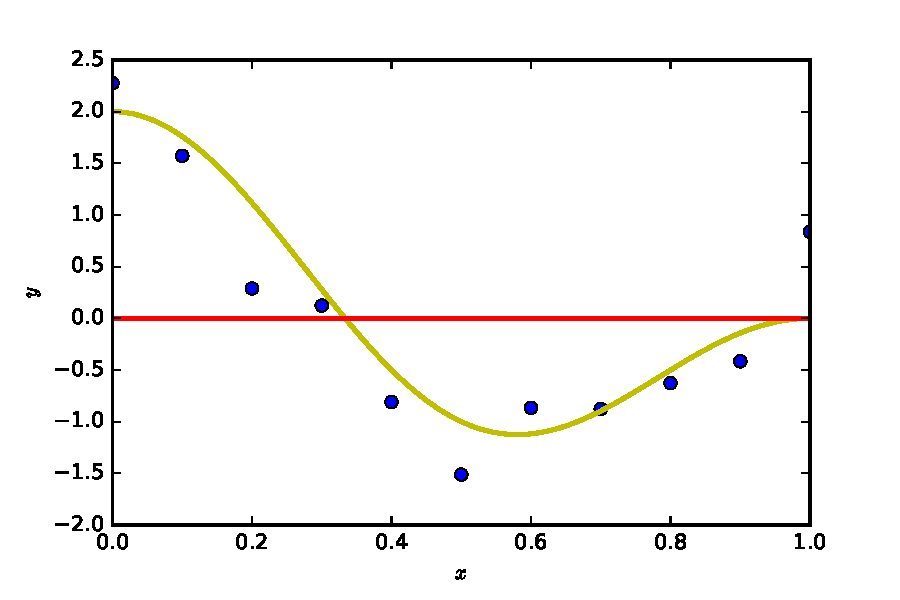
\includegraphics[width=3in]{img/2-1_degree0.pdf}  % $PLACEHOLDER
   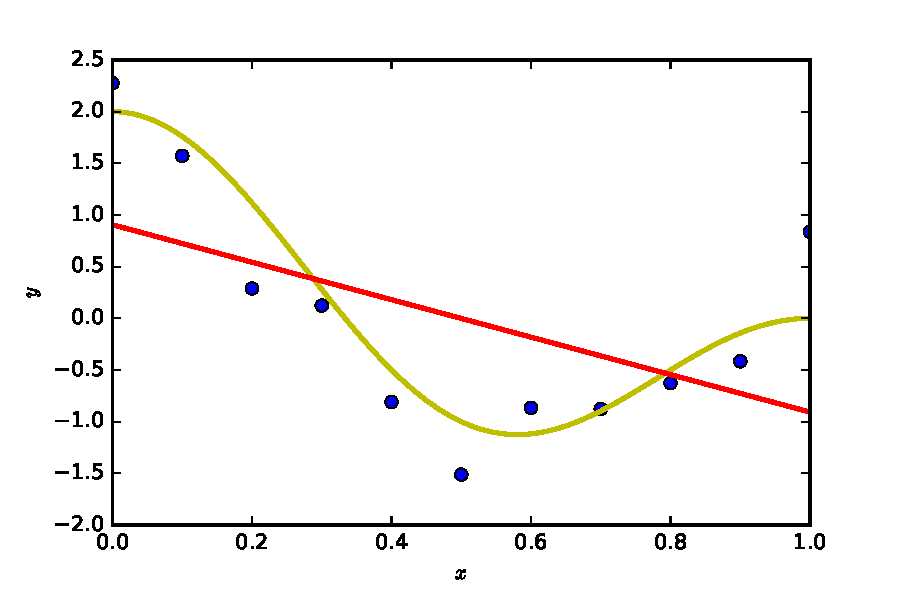
\includegraphics[width=3in]{img/2-1_degree1.pdf}  % $PLACEHOLDER
   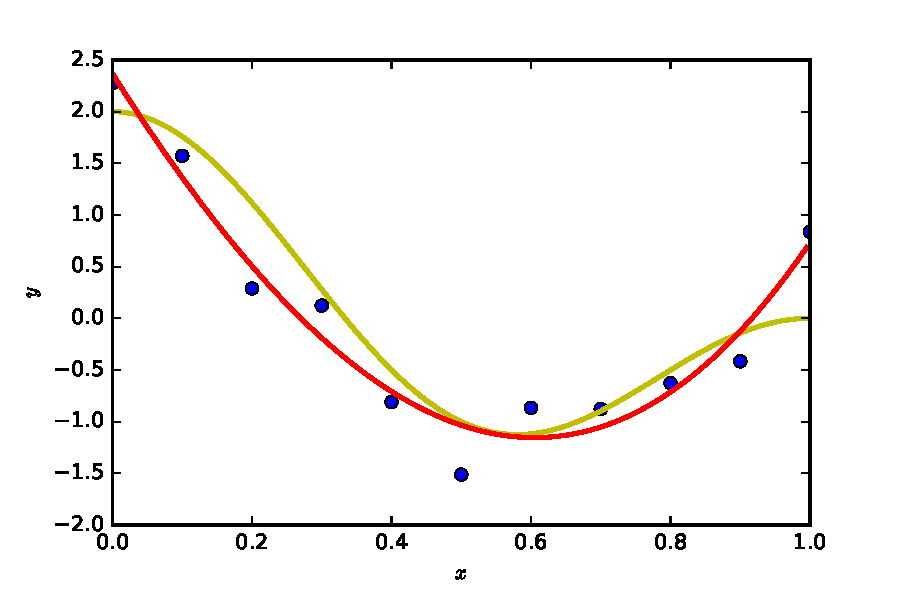
\includegraphics[width=3in]{img/2-1_degree3.pdf}  % $PLACEHOLDER
   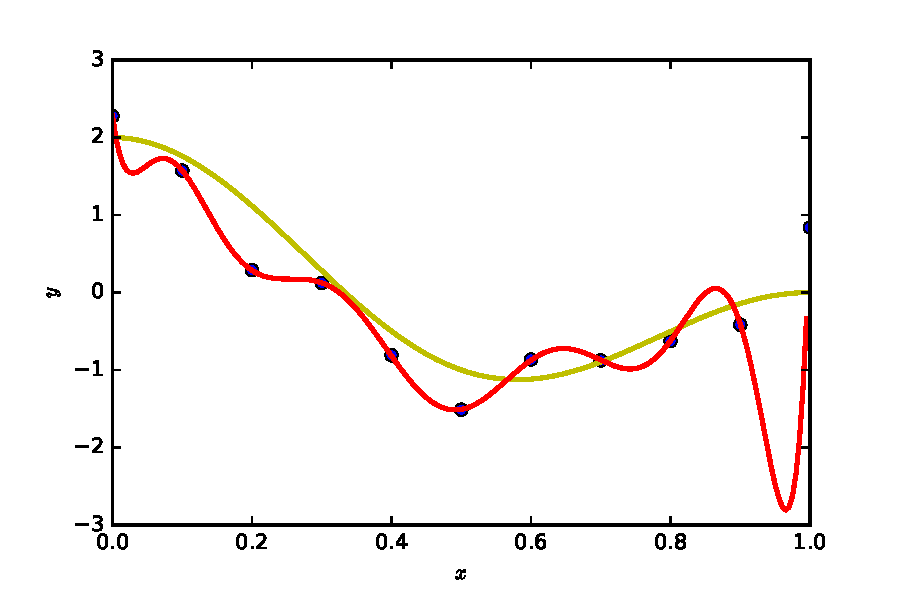
\includegraphics[width=3in]{img/2-1_degree10.pdf}  % $PLACEHOLDER
   \caption{Plots of our polynomial basis fits for degrees $M=0,1,3,10$ (red) of our dataset (blue), which was generated from an underlying function (yellow).
   The degree ascends from top to bottom, and within each row, from left to right.}
   \label{fig:2.1-polybasis}
\end{figure*}

\subsection{Regression by Gradient Descent}

Though there is a closed-form formula for the best-fit weight vector (Equation~\ref{eq:max-likelihood-weights}), we decided to verify our results from the previous section through gradient descent.

To this end, we considered the sum-of-squares error (SSE) for our problem:
\begin{align*}
J(w) &= \f12 \sum_n \lt(y^{(n)} - \sum_j\phi_j(x^{(n)}) w_j\rt)^2 \\
&= \f12 (\Phi w - Y)^T(\Phi w - Y), \label{eq:sse}\numberthis
\end{align*}
which has gradient
\beq
\label{eq:sse-grad}
\nabla J(w) = \Phi^T(\Phi w - Y).
\eeq
Using our numeric gradient approximation from section~\ref{subsec:grad-approx} (Equation~\ref{eq:grad-approx}), we verified the correctness of Equation~\ref{eq:sse-grad}.

We proceeded to estimate the maximmum-likelihood weight vector $w_\tx{ml}$ (Equation~\ref{eq:max-likelihood-weights}), which minimizes $J(w)$, using batch gradient descent on the SSE.
For small degree fits, the results agreed strongly with the closed-form solution.
However, for higher degrees, the discrepancies between our maximum-likelihood fits and our gradient-descent estimate fits grew progressively larger (Figure~\ref{fig:bgd-poly-fits}).

\begin{figure*}[h]
   \centering
   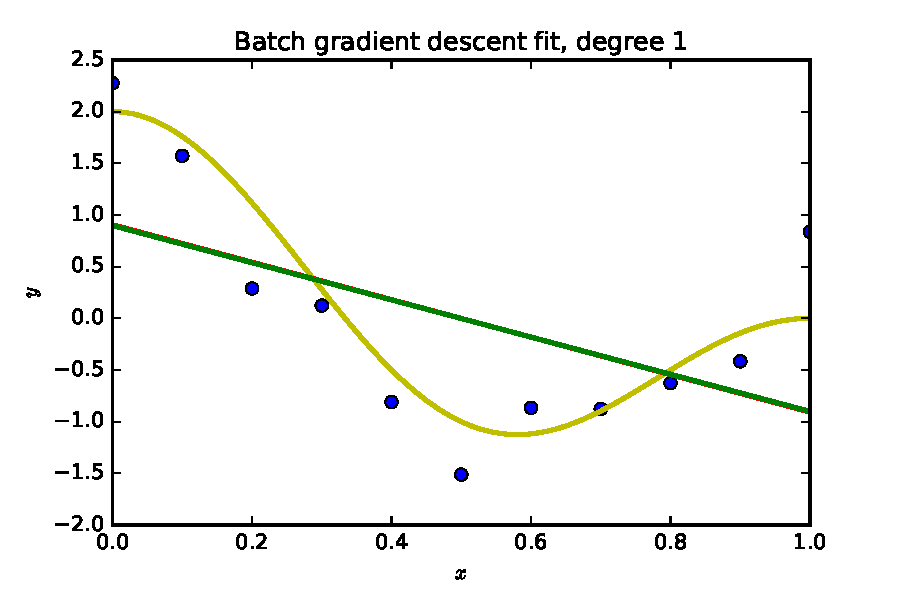
\includegraphics[width=2in]{img/2-3_bgd_fit_degree1.pdf}
   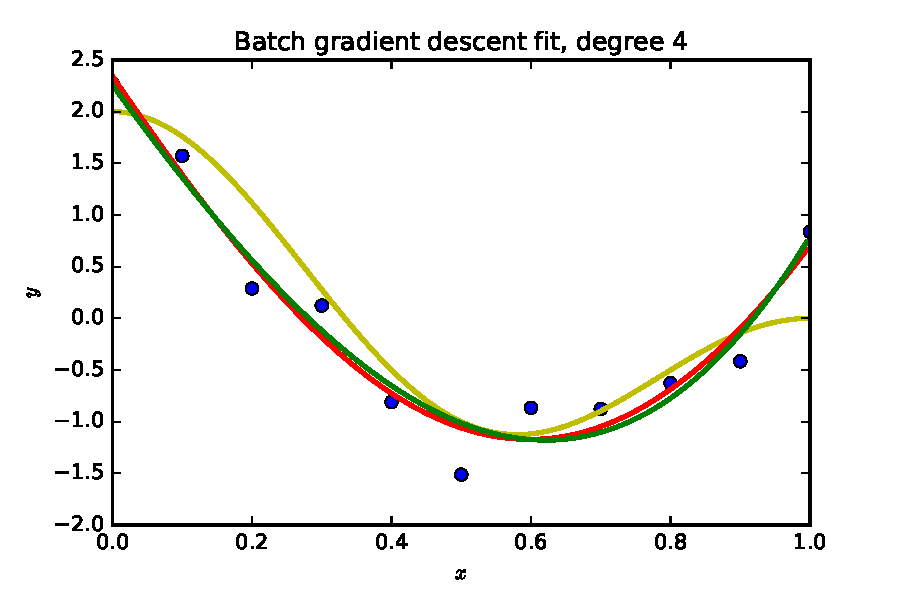
\includegraphics[width=2in]{img/2-3_bgd_fit_degree4.pdf}
   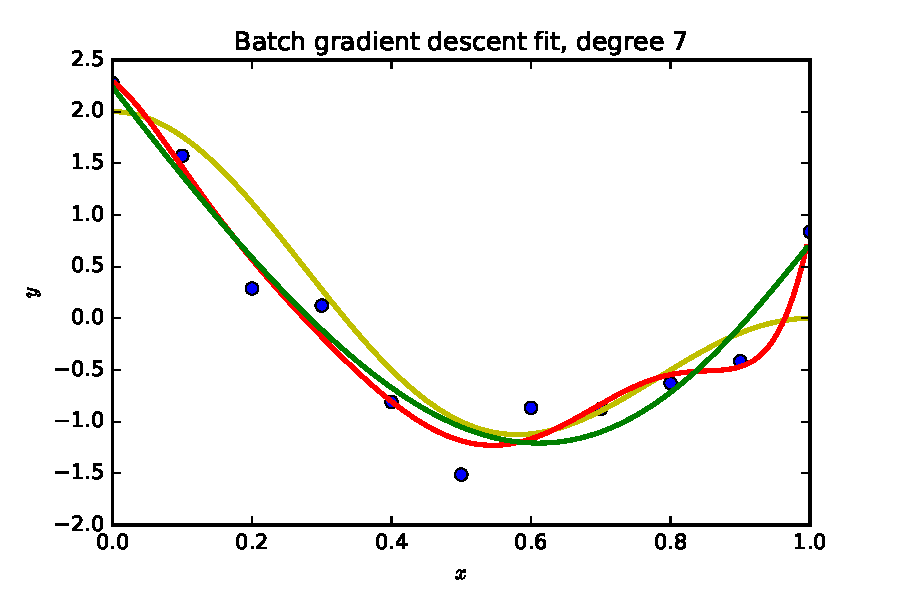
\includegraphics[width=2in]{img/2-3_bgd_fit_degree7.pdf}
   \caption{Polynomial fits of various degrees by batch gradient descent (green) of the dataset (blue) generated from a sum of cosines (yellow).
   The fits agree perfectly with the maximum-likelihood fits (red) at low degrees, but differ increasingly for higher degrees.
   Weights were initialized to zero.
   }
   \label{fig:bgd-poly-fits}
\end{figure*}

Interestingly, the gradient descent fits did not overfit nearly as much as the maximum-likelihood fits at high degree.
We conjecture that this behavior arises because we initialize our weight vectors at 0, ``regularizing" our fits in a sense.
Indeed, initializing our weight vectors to very large (in absolute value) random numbers produced wildly varying polynomials as fits.

Moreover, our gradient descent procedure terminates when the objective function changes between gradient descent iterations drops below a certain threshold, which we can think of as a form of early stopping.
Intuitively, overfitting requires a large change in our model parameters to get small decreases in our loss function; our convergence criterion prevents this sort of micro-optimization from occurring.

Varying step size had little effect at any degree.
Larger step sizes led to marginally faster convergence; overly large step sizes, however, led to divergence.
Varying the convergence threshold did not change our results significantly either (unless we set them unreasonably small or large).

We repeated this analysis with stochastic gradient descent (SGD), which was much more sensitive to the initial guess we provided.
Unless we initialized our weights closed to the correct (maximum-likelihood) value, SGD produced very poor fits at any degree.
At higher degrees, even picking initial weights close to their correct value did not seem to help with convergence.

This behavior can be explained if we consider the size of our dataset.
With a small dataset, it is more likely that the algorithm will believe it has converged when it hasn't, since it is conceivable that we terminate after checking a point that is already fit well and noticing that the resulting weight update changes the objective function very little.


\subsection{Cosine Basis Functions}

We also experimented with using cosine basis functions $\phi_m(x) = \cos(m\pi x)$ to fit the dataset.
Recall that the values were generated from Equation~\ref{eq:dataset-secret-func}, so we expect our weights to be $(0, 1, 1, 0, \dots)$ (recall that the first term is the weight for $\phi_0(x) \equiv 1$, so it is a bias term).
With a fit degree of~8, however, we overfitted significantly, and our weight vector differed greatly from the actual weights used to generate the data.

% elaborate??


% % % % % % % % % %
%    PROBLEM 3
% % % % % % % % % %

\section{Ridge Regression}

Recall that ridge regression is just linear regression, with an $L^2$ regularization term added to the loss function. That is, our error is the following modified version of Equation~\ref{eq:sse} (Bishop Equation~3.27):
\begin{equation}\label{eq:moderr}
J(w) = \f12 (\Phi w - Y)^T (\Phi w - Y) + \f12 \lambda ||w_+||^2,
\end{equation}
where $w_+$ is the vector of weights $w$ \emph{without} the bias term and $\lambda\ge 0$ controls the strength of regularization. So now we are penalizing large weights.

Then it can be shown that the optimal weight vector is given by
\begin{equation}
\label{eq:ridge-weights}
w_{+,\tx{ridge}} = (\lambda I + Z^T Z)\inv Z^T Y_c
\end{equation}
where $Z=\Phi - \overline\Phi$, where $\Phi$ is taken with \emph{no} column of 1's, and where $\overline\Phi$ is the average of all rows of $\Phi$ (an average of data points); and where $Y_c$ is $Y - \bar Y$, where $\bar Y$ is the mean of $Y$; and bias term
\begin{equation}
\label{eq:ridge-bias}
w_{0, \tx{ridge}} = \overline Y - w_{+,\tx{ridge}}^T \overline \Phi
\end{equation}


We implemented ridge regression and tested it on the data from our previous experiments on regression for a variety of polynomial degrees and values of $\lambda$. We present some of the fits in Figure~\ref{fig:ridge}.

\begin{figure*}[p] %  figure placement: here, top, bottom, or page
   \centering
   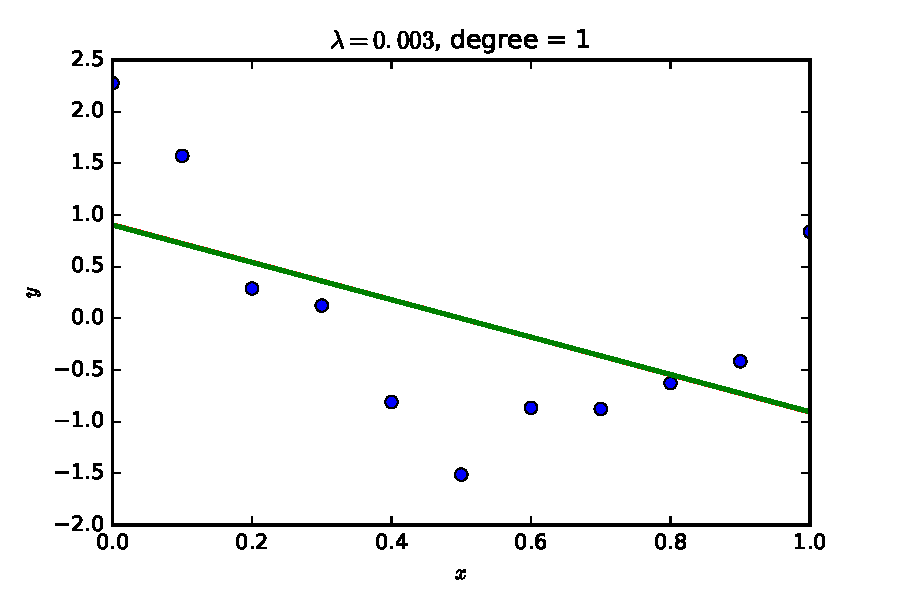
\includegraphics[width=3in]{img/3-1_ridge_lambd3_degree1.pdf}
   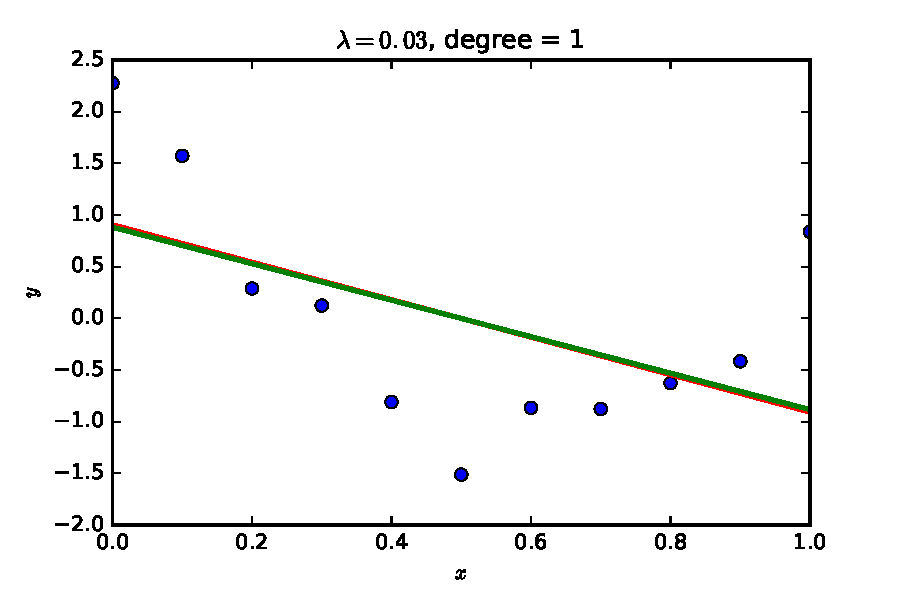
\includegraphics[width=3in]{img/3-1_ridge_lambd30_degree1.pdf}
   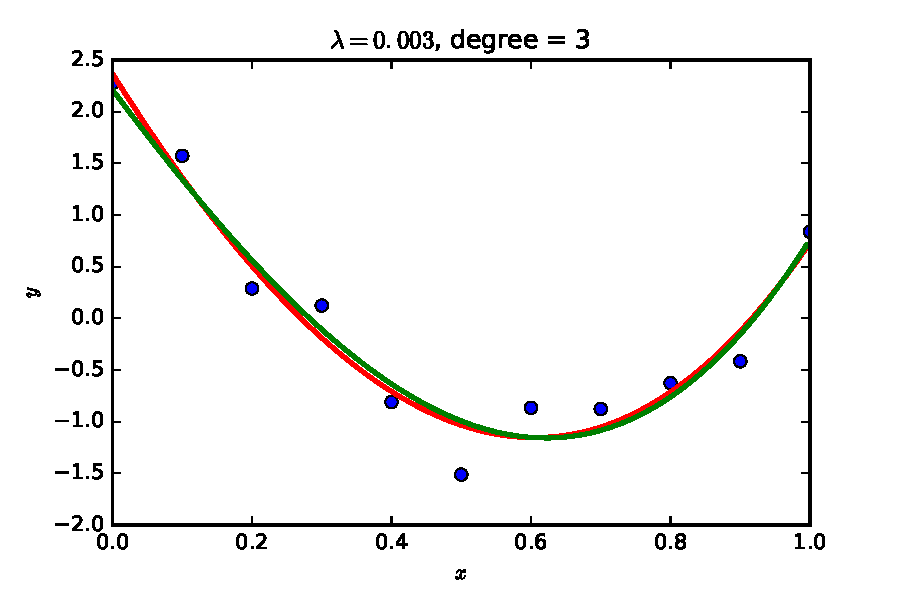
\includegraphics[width=3in]{img/3-1_ridge_lambd3_degree3.pdf}
   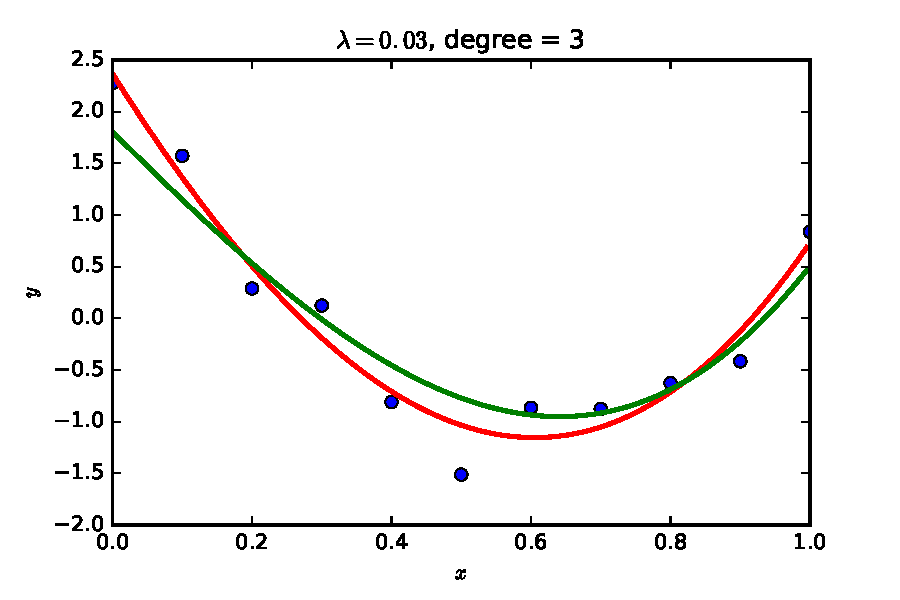
\includegraphics[width=3in]{img/3-1_ridge_lambd30_degree3.pdf}
   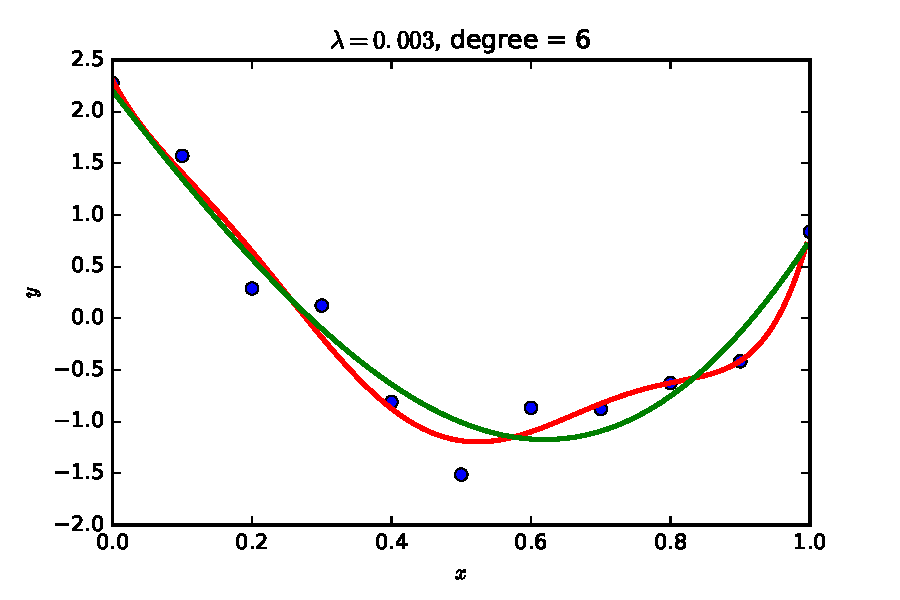
\includegraphics[width=3in]{img/3-1_ridge_lambd3_degree6.pdf}
   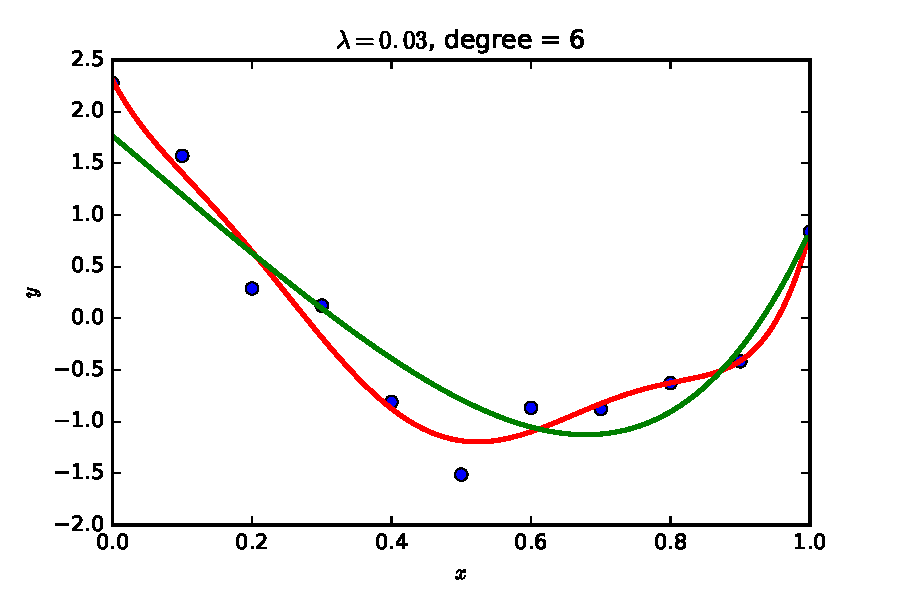
\includegraphics[width=3in]{img/3-1_ridge_lambd30_degree6.pdf}
   \caption{Regularized (green) and non-regularized (red) polynomial fits for the dataset from the previous section.}
   \label{fig:ridge}
\end{figure*}

Note that when fitting with higher order polynomial bases, even small values of $\lambda$ can drastically reduce overfitting. In general, at all degrees, larger values of $\lambda$ ``smooths" out and slightly ``flattens" our fit. Indeed, in the linear case, larger values of $\lambda$ would decrease the weight, i.e. the slope of our regression line.


\subsection{Model Selection}

We now turn our attention to another dataset, again of pairs of real numbers. This dataset has already been partitioned into sets $A$, $B$, and $V$, with respective sizes 13, 10, and 22. We will use $V$ as our validation set. We will try to model this data with a polynomial fit, as before, except we will be using regularization.

We used $A$ as training data and $B$ as test data, then vice versa.
In each case, we found the optimal weights using Equations~\ref{eq:ridge-weights} and \ref{eq:ridge-bias} on the training data for many values of the degree $M$ of the polynomial basis and the regularization parameter $\lambda$. We picked the pair $(M^*, \lambda^*)$ that produced the weight vector with the best performance on the \emph{validation} data, then evaluated the model they produced on the test data.
Note that we evaluate performance of an actual weight vector with ordinary mean-square error (MSE; Equation~\ref{eq:sse}, but normalized by the number of data points), with \emph{no regularization term}.

We present validation errors for a variety of $M$ and $\lambda$ in Tables~\ref{tab:val-mse-a} and \ref{tab:val-mse-b}.
When we trained on $A$ and tested on $B$, the hyperparameters that produced the smallest MSE on validation were $(M^*,\lambda^*)=(2,0)$; the MSE was $0.05336$. On test data $B$, the same model achieved an MSE of $1.28765$.
When we trained on $B$ and test on $A$, the best hyperparameters $(M^*,\lambda^*)=(3,0.6)$ produced a validation error of $0.65195$. The test error on the same model was $1.51697$.
We plot these two best-fit models in Figure~\ref{fig:3-2-bestfit}.


\begin{table*}
\caption{Mean-square error on our validation set after training on $A$. The optimal pair of hyperparameters was $(M^*,\lambda^*) = (2, 0)$.}
\centering
\begin{tabular}{|l||c|c|c|c|c|c|}
\hline
\backslashbox{$\lambda$}{$M$} & 0		& 1		 & 2	   & 3 & 4 & 5 \\\hline
0		& 1.40909 & 0.06584 & {\color{red}0.05336} & 0.05386 &  0.08134  & 0.09403\\
0.001	& " & 0.06584 & 0.05336 & 0.05388 &0.08129& 0.09393\\
0.003	& " & 0.06585 & 0.05337 & 0.05392 &0.08119& 0.09373\\
0.01	& " & 0.06587 & 0.05339 & 0.05407 &0.08086& 0.09305\\
0.03	& " & 0.06596 & 0.05345 & 0.05450 &0.07998& 0.09120\\
0.1		& " & 0.06624 & 0.05366 & 0.05600 &0.07747& 0.08564\\\hline
\end{tabular}
\label{tab:val-mse-a}
\end{table*}

\begin{table*}
\caption{Analogous to Table~\ref{tab:val-mse-a}, except with training on $B$. The best hyperparameters are $(M^*,\lambda^*)=(3,0.6)$.}
\centering
\begin{tabular}{|l||c|c|c|c|c|c|}
\hline
\backslashbox{$\lambda$}{$M$}&
0		& 1		 & 2	   & 3 & 4 & 5 \\\hline
0		& 1.64635 & 0.79978 & 0.87563 & 0.68864 &  2.95901  & 14.21443\\
%0.001	& " & 0.79981 & 0.87562 & 0.68843 & 2.95298 & 14.17389\\
%0.003	& " & 0.79987 & 0.87560 & 0.68801 & 2.94101 & 14.09364\\
%0.01	& " & 0.80008 & 0.87553 & 0.68656 & 2.89993 & 13.82113\\
0.03	& " & 0.80066 & 0.87533 & 0.68262 & 2.78933 & 13.10785\\
0.1		& " & 0.80271 & 0.87471 & 0.67110 & 2.46809 & 11.18677\\
0.3		& " & 0.80852 & 0.87347 & 0.65314 & 1.90417 & 8.20467\\
0.6		& " & 0.81709 & 0.87289 & \color{red}0.65195 & 1.51048 & 6.18385\\
1.0		& " & 0.82828 & 0.87410 & 0.67289 & 1.29261 & 4.82707
\\\hline
\end{tabular}
\label{tab:val-mse-b}
\end{table*}

\begin{figure*}
   \centering
   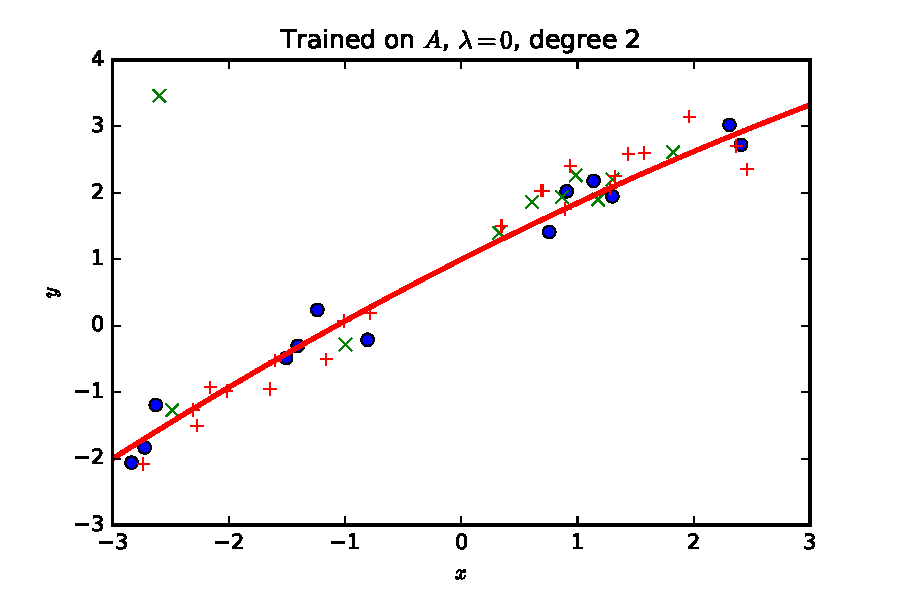
\includegraphics[width=3in]{img/3-2_lambda0_degree2.pdf} 
   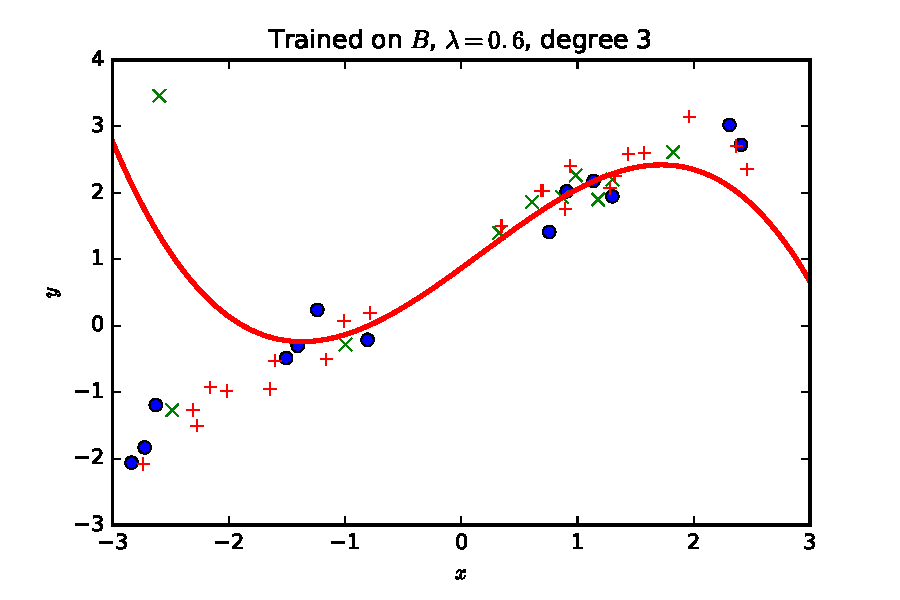
\includegraphics[width=3in]{img/3-2_lambda6_degree3.pdf} 
   \caption{Best fit models for our dataset, where $A$ is plotted with blue dots, $B$ with green crosses, and $V$ with small plus signs. Note how the single outlier in $B$ skews the second fit significantly.}
   \label{fig:3-2-bestfit}
\end{figure*}

Before concluding this section, we observe from Tables~\ref{tab:val-mse-a} and \ref{tab:val-mse-b} that increasing the degrees of freedom in our model increases the optimal value of $\lambda$.


% % % % % % % % % %
%    PROBLEM 4
% % % % % % % % % %

\section{Sparsification with LASSO}

% #PLACEHOLDER
In previous parts, we have encountered relatively simple closed-form answers. However, that is not always the case; for problems without such solutions, we may estimate sparse weights with the LASSO (least absolute shrinkage and selection operation) method.

Recall that in ridge regression, we modified our error to include a quadratic regularizer. A more generalized form of Equation \ref{eq:moderr} (Bishop 3.29) can be extended to other exponents. In particular, when exponent $q=1$, we have the LASSO error function:
\begin{equation}J(w) = \f{1}{n}\sum_{i=1}^n{(y^{(i)}-w^T\phi(x^{(i)}))^2} + \lambda \sum_{j=1}^M{|w_j|}.\end{equation}

We implemented LASSO for basis given by
\begin{equation}\phi(x)=(x, \sin{(0.4\pi x\cdot1)},\dots,\sin{0.4\pi x\cdot 12})\in \mathbb{R}^{13}
\end{equation}
We compared its performance with that of ridge regression and observed that sparsity increases and some coefficients $w_j$ are driven to 0 as $\lambda$ increases. This is because, we are subject to the following constraint when minimizing the error function (Bishop 3.30):
\begin{equation}\sum_{j=1}^M{|w_j|} \le \eta.\end{equation}

\end{multicols}

\end{document}
